\setchapterimage[6cm]{seaside}
\setchapterpreamble[u]{\margintoc}
\chapter{Introduction en Français}
\labch{intro_french}

\section{L'égalité dans la Théorie des Types Intensionnelle}

Si vous avez déjà utilisé un assistant de preuve basé sur la théorie des types 
intensionnelle comme \Coq, \Agda ou \Lean---et il y a de fortes chances que 
ce soit votre cas si vous êtes en train de lire cette thèse---alors vous savez 
sans doute que l'égalité peut être un véritable casse-tête.

D'une part, nous avons l'égalité définitionnelle (également appelée conversion), 
qui enregistre les équations que l'assistant de preuve manipule silencieusement 
pour nous. 
% 
\sideremark{Dans un assistant de preuve basé sur la théorie des ensembles ZF 
  comme Metamath, le théorème \( {2+2=4} \) demande une preuve. 
  Et bien qu'elle soit élémentaire, cette preuve implique une quantité surprenante 
  de lemmes auxiliaires !}
% 
Par exemple, les termes \( 2 + 2 \) et \( 4 \) sont égaux défintionnellement, 
ce qui signifie que nous pouvons les utiliser indifféremment dans nos preuves 
sans avoir à nous soucier de prouver leur égalité à la main. 
% 
Lorsqu'on utilise des types dépendants, cette quantité minimale 
d'automatisation est absolument vitale ; pour éviter de se retrouver à insérer 
des coercitions explicites à chaque fois que nous voulons, par exemple, 
utiliser un terme de type \( \mathsf{Vector}\ (2+2) \) en tant que terme de 
type \( \mathsf{Vector}\ 4 \).

Mais malheureusement, il existe des objets qui ne sont pas des entiers 
naturels\sidenote{[référence nécessaire]}, et les preuves mathématiques traitent 
souvent d'égalités entre des objets infinitaires tels que les fonctions et les 
ensembles. 
% 
Et naturellement, il n'existe pas d'algorithme capable de décider si deux 
fonctions de type \( \Nat \to \Nat \) associent les mêmes images aux mêmes 
antécédants.
% 
Ainsi en pratique, l'égalité définitionnelle se limite aux égalités 
\( \beta / \eta / \iota \), avec possiblement quelques extensions comme les 
règles de réécriture d'Agda~\sidecite{taming_of_the_rew}.

Puisque le système ne sera pas en mesure d'automatiser complètement toutes 
les égalités, nous avons besoin d'un moyen de raisonner à leur sujet. 
% 
C'est pourquoi la théorie des types intensionnelle fournit une deuxième notion 
d'égalité, appelée l'égalité \emph{propositionnelle}.
% 
Contrairement à l'égalité définitionnelle, celle-ci est disponible 
dans le langage de la théorie des types, et nous pouvons l'utiliser 
pour énoncer et prouver des théorèmes. 
% 
Dans les trois principaux assistants de preuve basés sur la théorie des types, 
l'égalité propositionnelle est implémentée avec un type inductif, d'après les 
travaux de Martin-Löf~\sidecite{MartinLoef75}.
% 
\sideremark{L'égalité propositionnelle \( \Indeq{A}{t}{u} \) est un type, tandis
  que l'égalité définitionnelle \( \eqtm{\Gamma}{t}{u}{A} \) est un jugement de typage.}
\begin{mathpar}
  \inferrule{\tyty{\Gamma}{A}
			\\ \tytm{\Gamma}{t}{A}
			\\ \tytm{\Gamma}{u}{A}}
			{\tyty{\Gamma}{\Indeq{A}{t}{u}}}
  \and
  \inferrule{\tyty{\Gamma}{A}
			\\ \tytm{\Gamma}{t}{A}}
			{\tytm{\Gamma}{\indrefl{t}}{\Indeq{A}{t}{t}}}
\end{mathpar}
\begin{mathpar}
  \inferrule{\tyty{\Gamma}{A}
			\\ \tytm{\Gamma}{t}{A}
			\\ \tytm{\Gamma}{B}{\Depfun{A}{\Fun{t =_A x}{\Univ}}}
			\\ \tytm{\Gamma}{u}{B\ t\ \mathsf{refl}_t}
			\\ \tytm{\Gamma}{t'}{A}
			\\ \tytm{\Gamma}{e}{t =_A t'}}
			{\tytm{\Gamma}{\mathsf{J}(A,t,B,u,t',e)}{B\ t'\ e}}
\end{mathpar}
\begin{mathpar}
  \inferrule{[...]}
			{\red{\Gamma}{\mathsf{J}(A,t,B,u,t,\mathsf{refl}_t)}{u}{B\ t\ \mathsf{refl}_t}}
\end{mathpar}

Ces quelques règles suffisent à définir une relation d'équivalence qui contient 
l'égalité définitionnelle, peut être utilisée pour réécrire des termes et peut 
être utilisée pour convertir des termes entre deux types égaux.

Une différence importante avec la pratique courante des mathématiques est que nous restons 
très attachés à la correspondance de Curry-Howard entre les preuves et les programmes : 
l'égalité est un type, et les preuves d'égalité sont des programmes\sidenote{amen.}. 
% 
En tant que telles, les preuves d'égalité sont des valeurs de première classe 
tout comme les entiers naturels ou les fonctions, et elles sont donc sujettes 
au raisonnement mathématique, et elles peuvent également être évaluées.

\subsection{Types et Propositions}

Bien que la possibilité d'évaluer les preuves soit un principe fondamental de 
la philosophie Curry-Howard, une preuve d'égalité typique n'a pas un 
comportement calculatoire très intéressant. 
% 
Le terme \( \indJ{A}{t}{P}{u}{t'}{e} \) se contente d'attendre que \( e \) se 
réduise en une preuve par réflexivité, auquel cas \( t \) et \( t' \) sont 
convertibles et le terme entier peut simplement être évalué en \( u \).

Par conséquent, les programmes 
\defnote{extraits}{L'extraction produit un programme dans un langage externe
  en effaçant une partie des types.} 
à partir de preuves qui utilisent du raisonnement équationnel ont tendance à 
passer beaucoup de temps à propager les preuves d'égalité, pour finir par les 
effacer lorsqu'elles ne sont plus nécessaires. 
% 
Cette situation sous-optimale a conduit l'assistant de preuve de Coq à 
introduire une sorte spéciale \( \varProp \) pour les types dont les preuves sont 
effacées lors de l'extraction~\sidecite{letouzey04}. 
% 
En plaçant l'égalité propositionnelle dans \( \varProp \) avec les autres 
contraintes logiques qui ne jouent aucun rôle calculatoire, Coq retrouve des 
performances raisonnables pour les programmes extraits.

Techniquement, c'est un peu une violation de la discipline de Curry-Howard, 
puisque \( \varProp \) réintroduit une séparation entre les propositions et les données.
%  
Mais ne vous méprenez pas : les preuves de propositions jouent encore
leur rôle normal dans les calculs de théorie des types, et en particulier, 
elles peuvent bloquer l'évaluation des termes ouverts. 
% 
C'est seulement lorsque nous extrayons un programme \emph{externe} que les 
propositions sont effacées.

L'assistant de preuve \Lean va un peu plus loin et introduit la sorte 
\( \varsProp \) pour les \emph{propositions strictes}~\sidecite{lean}. 
% 
Contrairement aux propositions de \Coq, les propositions strictes sont
\emph{proof-irrelevant}, ce qui signifie que deux habitants quelconques 
d'une proposition stricte \( A \) sont définitionnellement égaux.
% 
\[
\inferrule{\tytm{\Gamma}{A}{\varsProp} \\ \tytm{\Gamma}{t, u}{A}}{\eqtm{\Gamma}{t}{u}{A}}
\]

Mettre l'égalité propositionnelle dans \( \varsProp \) n'est pas aussi inoffensif 
qu'il n'y parait.
% 
En particulier, cela implique que toute preuve d'égalité propositionnelle entre 
deux termes convertibles est maintenant indiscernable d'une preuve par réflexivité 
(puisque les deux preuves ont le même type). 
% 
En d'autres termes, \Lean satisfait une version stricte du principe de 
\emph{uniqueness of identity proofs} (UIP).

Avec ce principe, les preuves d'égalité non-réflexives ne sont plus capables de 
bloquer un calcul : le terme \( \indJ{A}{t}{P}{u}{t}{e} \) est convertible en 
\( \indJ{A}{t}{P}{u}{t}{\indrefl{t}} \), qui devrait se réduire !
% 
Par conséquent, l'éliminateur \( J \) de \Lean se réduit dès qu'il est appliqué 
à deux termes définitionnellement égaux.
\begin{mathpar}
  \inferrule[J-conv]{[...] \\ \eqtm{\Gamma}{t}{t'}{A}}
			{\red{\Gamma}{\mathsf{J}(A,t,B,u,t',e)}{u}{B\ t'\ e}}
      \ilabel{infrule:J-conv}
\end{mathpar}

Mais bien que cette règle soit logiquement cohérente, Abel et Coquand ont montré 
qu'elle conduit à un échec de la normalisation pour les termes 
ouverts~\cite{lmcs:6606}. 
% 
\sideremark{Il est établi que l'égalité définitionnelle de \Lean est indécidable
  pour des raisons orthogonales~\cite{gilbert:hal-01859964}. Toutefois, 
  remarquons que ça n'a pas empêché la communauté de \Lean de développer 
  une impressionante quantité de mathématiques.}
% 
Et comme les algorithmes que nous utilisons pour vérifier la convertibilité 
reposent sur la normalisation, on en déduit que l'ajout de la 
règle~\nameref{infrule:J-conv} casse notre procédure de décision pour l'égalité 
définitionnelle. 
% 
Comme l'ont remarqué Abel et Coquand, il n'est pas clair que cela provienne d'une 
incompatibilité fondamentale entre les propositions strictes imprédicatives et 
l'égalité propositionnelle, et qu'il n'existe pas une stratégie plus 
intelligente qui pourrait résoudre ce problème.

\subsection{Imprédicativité}

En théorie des types dépendants, une sorte est dite \emph{imprédicative} 
quand elle est close par produits dépendants indexés par n'importe quel type. 
% 
Par exemple la sorte des propositions de \Coq est imprédicative, car pour tout 
type \( A \) et toute fonction \( \tm{B}{A \to \varProp} \) le produit dépendant 
\( \Depfun{A}{B\ x} \) est dans \( \varProp \).

L'imprédicativité introduit de l'autoréférence dans notre système 
de types : nous pouvons l'utiliser pour former une proposition \( P \) qui 
quantifie sur le type \( \varProp \) de toutes les propositions, type qui 
contient \( P \). 
% 
Un exemple classique est l'encodage imprédicatif de la proposition fausse, 
dont les habitants peuvent être éliminés dans n'importe quelle autre proposition :
\[
\Depfun[X]{\varProp}{X} \quad : \quad \varProp
\]

Comparez cette situation avec la hiérarchie \emph{prédicative} 
$(\varType_i)_{i \in \Nat}$ 
% 
\sideremark{Dans l'assistant de preuve \Coq, les univers prédicatifs ne sont 
  techniquement pas indexés par des entiers, mais le système maintient un graphe
  de contrainte de niveau d'univers qui remplit la même fonction.}
% 
des types non-propositionnels.
% 
Dans le monde non-propositionnel, les produits dépendants sont forcés de vivre 
dans un niveau d'univers qui est à la fois plus grand que celui de leur domaine et
plus grand que celui de leur codomaine :
% 
étant donné un type \( A : \varType_i \) et une fonction \( {\tm{B}{A \to \varType_j}} \), 
le produit dépendant \( \Depfun{A}{B\ x} \) atterrit dans l'univers
\( \varType_{\mathsf{max}(i,j)} \).
 
La prédicativité supprime les possibilités d'autoréférence : si nous essayons 
de reproduire l'encodage de la proposition fausse dans \( \varType_0 \), le 
type résultant se retrouve dans l'univers \( \varType_1 \).
\[
\Depfun[X]{\varType_0}{X} \quad : \quad \varType_1
\]

Autoriser l'autoréférence revient à jouer avec le feu : les antinomies 
logiques héritées du paradoxe de Russell restent tapies dans l'ombre, et 
pourraient nous attraper si nous sommes un peu trop gourmands avec nos 
règles logiques.
% 
Par exemple, le paradoxe de Berardi montre qu'avoir le tiers exclu et les 
l'élimination large pour les booléens à valeur dans \( \varProp \) est incohérent. 
% 
L'imprédicativité joue également un rôle central dans le terme 
non-normalisant qu'Abel et Coquand ont obtenu à partir de la 
règle~\nameref{infrule:J-conv}~\sidecite{lmcs:6606}.

En contrepartie pour cette fragilité, l'imprédicativité augmente considérablement 
le pouvoir expressif de notre système logique, et nous permet de formuler 
d'importantes constructions mathématiques telles que le théorème du point fixe 
de Tarski ou des treillis complets non-triviaux~\sidecite{paco}. 
% 
De plus, certains théorèmes comme la normalisation du Système F ne peuvent tout
simplement pas être prouvés dans une théorie prédictive.

Les différents assistants de preuve ont adopté des attitudes variées envers 
l'imprédicativité. D'un côté, 
% 
\sideremark{Fut un temps, \Coq utilisait également une sorte imprédicative
  pour les types \emph{proof-relevant}, mais l'équipe de développement a 
  préféré désactiver cette fonctionnalité pour avoir une théorie plus proche
  des mathématiques classiques.}
% 
\Coq et \Lean ont tous deux adopté l'imprédicativité pour leur sorte des 
propositions, qui cohabite avec la hiérarchie d'univers prédicatifs utilisée 
pour les types \emph{proof-relevant}~\sidecite{Coq:manual,lean}.
% 
De l'autre côté, l'assistant de preuve \Agda a choisi de ne pas implémenter
l'imprédicativité et utilise deux hiérarchies prédicatives à la place, une 
pour les propositions strictes et une pour les types~\sidecite{agda261}.

\section{L'Extensionalité dans la Théorie des Types Intensionnelle}

L'égalité propositionnelle simple que nous avons définie avec un type inductif 
ne répond pas vraiment aux exigences du raisonnement mathématique. 
% 
En mathématiques, deux fonctions sont considérées comme égales lorsqu'elles 
coïncident sur tous les antécédants---il s'agit du principe 
d'\emph{extensionnalité des fonctions}---mais
% 
\sideremark{En particulier, il est impossible de montrer que les fonctions
\( {\lambda\ n\ .\ n+1} \) and \( {\lambda\ n\ .\ 1+n} \) sont égales.}
% 
ce principe n'est pas démontrable pour l'égalité propositionnelle dans 
la théorie des types intensionnelle.
\[
  \Indeq{A \to B}{f}{g} \quad \xcancel{\longleftrightarrow} \quad \Depfun{A}{\Indeq{B}{f\ x}{g\ x}}
\]

En fait, nous pouvons même prouver que toutes les preuves d'égalité 
propositionnelle dans un contexte clos se réduisent à l'égalité définitionnelle. 
% 
C'est une conséquence directe de la normalisation des termes bien typés : 
la seule forme normale close pour une preuve d'égalité est \( \indrefl{t} \), 
terme qui n'est typable que si les deux membres de l'égalité sont convertibles. 
% 
Et comme nous l'avons expliqué précédemment, l'égalité définitionnelle est 
incapable de gérer l'égalité naturelle des fonctions. 

Développer des mathématiques complexes sans le principe d'extensionnalité 
des fonctions n'est pas une tâche facile. Par conséquent, notre communauté a 
considéré plusieurs options pour retrouver une égalité plus conventionnelle au 
fil des ans.

\paragraph*{Postuler des axiomes d'extensionnalité}
% 
Le moyen le plus simple de récupérer un principe de raisonnement manquant 
est simplement de le postuler comme axiome. 
% 
\sideremark{Remarquons qu'avec \Coq et \Lean, il est possible d'extraire un 
  programme à partir d'une preuve qui postule l'axiome d'extensionnalité des
  fonctions, puisque cet axiome est une proposition et sera donc effacé lors
  de l'extraction.}
% 
Par exemple, l'axiome \textsf{functional\_extensionality\_dep} est disponible 
dans la bibliothèque standard de Coq. 
% 
L'utilisation d'axiomes a toutefois des inconvénients, car ils ne se comportent 
pas très bien vis-à-vis des propriétés calculatoires de la théorie des types 
intensionnelle : appliquer l'éliminateur \( \mathsf{J} \) à une égalité obtenue 
via un axiome ne produira qu'un terme bloqué.

\paragraph*{Utiliser des sétoïdes}
% 
Une technique standard pour récupérer les principes d'extensionnalité sans entrer
en conflit avec la correspondance preuves-programmes est d'utiliser des 
\emph{sétoïdes}~\sidecite{hofmann95}, c'est-à-dire de remplacer les types par 
des couples \( (|A|, e_A) \) d'un type \( |A| \) et d'une relation d'équivalence 
\( e_A \) sur \( |A| \) (l'\emph{égalité sétoïdale} de \( A \)).
% 
Nous pouvons alors considérer uniquement les fonctions qui préservent l'égalité 
sétoïdale, et nous pouvons demander l'extensionnalité dans l'égalité sétoïdale 
des types de fonctions.

Travailler avec des sétoïdes n'est pas très agréable, car nous devons accompagner 
chaque définition par des preuves bureaucratiques de préservation de l'égalité
sétoïdale, alors même que toutes les constructions possibles en théorie des types 
respectent naturellement l'extensionnalité des fonctions~\sidecite{Altenkirch99}. 
% 
En un mot, nous devons faire le travail d'un compilateur à la main. 
% 
\Coq implémente des tactiques pour traiter les sétoïdes plus efficacement, mais 
elles supportent difficilement le passage à l'échelle de développements conséquents---
au point que la communauté utilise le terme \emph{setoid hell} en référence à ces 
problèmes.

\paragraph*{Changer la théorie}
% 
Étant donné que les axiomes d'extensionnalité sont problématiques parce qu'ils 
bloquent le calcul, les théoriciens des types ont envisagé plusieurs manières 
d'étendre la théorie des types intensionnelle avec de nouvelles règles de calcul 
pour gérer les axiomes souhaités. 
% 
Les travaux les plus fructueux peuvent être divisés en deux groupes : d'une part ceux qui 
remplacent l'égalité propositionnelle inductive par une 
\emph{égalité observationnelle}, et d'autre part ceux qui la remplacent par une 
\emph{égalité univalente}.

\subsection{L'Égalité Observationnelle}

Les origines de l'égalité observationnelle remontent aux travaux de Hofmann et 
Altenkirch sur le modèle sétoïdal de la théorie des types~\cite{hofmann95,altenkirch99}.
% 
En interprétant les types comme des sétoïdes, ils ont pu modéliser
\defnote{ITT+funext}{ITT+funext est une abréviation pour la théorie des types intensionnelle 
avec l'axiome d'extensionalité des fonctions.}
dans une théorie des types intensionnelle étendue avec des propositions strictes. 
Étant donné que ces propositions strictes n'entrent pas en conflit avec l'interprétation 
des preuves en tant que programmes, le modèle sétoïdal fournit un moyen d'évaluer les 
preuves qui utilisent l'axiome d'extensionnalité des fonctions, en évaluant leur 
interprétation.

L'ingrédient central du modèle sétoïdal est l'interprétation de l'univers. 
% 
Construire un sétoïde qui contient tous les petits sétoïdes semble difficile 
en première approche, car la collection de tous les petits sétoïdes n'a pas 
d'égalité sétoïdale naturelle ; mais cela peut être résolu en utilisant un univers 
\defnote{inductif-récursif}{L'induction-recursion est un principe logique puissant qui 
  permet de définir un type inductif \( A \) simultanément avec des fonctions
  définies par récursion sur \( A \).} 
de codes sur lequel on définit récursivement l'égalité sétoïdale 
ainsi qu'un opérateur de \emph{type-casting}.

Suite à cette première étape, Altenkirch McBride et 
Swierstra~\sidecite{altenkirchAl:plpv2007} ont développé la théorie des types 
observationnelle (OTT), une extension de la théorie des types intensionnelle 
qui ramène les idées du modèle sétoïdal dans le monde de la syntaxe : 
% 
OTT incorpore un nouvel opérateur primitif appelé 
\emph{égalité observationnelle} qui dote chaque type d'une structure de sétoïde 
définie par récursion sur l'univers. 
% 
Grâce à cela, OTT implémente les principes d'UIP et d'extensionnalité des 
fonctions, et de plus Altenkirch \etal prouvent que la normalisation des termes 
OTT découle d'un résultat de normalisation conjecturé pour la théorie des types 
avec induction-récursion.

L'égalité observationnelle a connu un certain renouveau ces dernières années, 
avec notamment les travaux de Sterling et al. qui la revisitent sous l'angle 
de la théorie des types cubique~\sidecite{sterling-angiuli-gratzer:2022} ou bien
les travaux sur \emph{setoid type theory} d'Altenkirch \etal~\sidecite{Altenkirch2019}. 
% 
Toutefois, la théorie des types observationnelle n'a pas encore atteint un niveau 
de maturité comparable à celui des théories des types univalentes. 
% 
En particulier, il n'existe toujours pas de support pour l'égalité 
observationnelle dans les principaux assistants de preuve, bien que des
travaux aient été menés dans cette direction~\sidecite{mcbride-autopsy}.

\subsection{L'Égalité Univalente}

La seconde famille de travaux, plus récente, remonte à la formulation de
l'\emph{axiome d'univalence} de Voevodsky~\sidecite{kapulkin2012simplicial,hottbook}.
\[
(A =_{\varType} B) \enskip \simeq \enskip  (A \simeq B)
\]

L'axiome d'univalence donne un sens nouveau à l'égalité entre les types : 
% 
\sideremark{Donner une bonne définition d'un isomorphisme entre deux types est
  plus subtil qu'il n'y paraît. Pour éviter trop de digressions dans notre 
  introduction, nous supposerons que cette définition nous est donnée.}
% 
se donner un témoin d'égalité entre \( A \) et \( B \) revient à se donner un 
élément du type \( A \simeq B \) des \emph{isomorphismes} entre \( A \) et \( B \). 
% 
L'univalence peut être vue comme un principe d'extensionnalité pour l'univers 
des types, et l'ajouter à la théorie des types intensionnelle entraîne des 
conséquences remarquables. 
% 
En particulier, l'axiome d'univalence implique le principe d'extensionnalité des 
fonctions.

\paragraph*{La Théorie des Types Homotopique}
% 
L'axiome d'univalence s'éloigne de l'usage habituel de l'égalité en mathématiques,
en ce sens que l'égalité ne peut plus être une proposition puisqu'elle contient 
désormais des informations essentielles pour le calcul.  
% 
Par exemple, il existe deux automorphismes distincts du type des booléens---l'un 
correspondant à l'identité et l'autre à la négation---et transporter un terme avec 
l'identité ne donne pas les mêmes résultats que le transport avec la négation.
% 
\sideremark{Transporter une terme \( t : A \) avec un isomorphisme \( f : A \simeq B \) 
  revient à appliquer l'isomorphisme à \( t \), à une égalité propositionnelle près.}
\[
\begin{split}
\indJ{\varType}{\mathsf{Bool}}{\lambda X\ .\ X}{\mathsf{true}}{\mathsf{Bool}}{\mathsf{id}} & \enskip =_{\mathsf{Bool}} \enskip \mathsf{true} \\
\indJ{\varType}{\mathsf{Bool}}{\lambda X\ .\ X}{\mathsf{true}}{\mathsf{Bool}}{\mathsf{neg}} & \enskip =_{\mathsf{Bool}} \enskip \mathsf{false}
\end{split}
\]

Ainsi lorsque nous utilisons l'axiome d'univalence, nous devons accepter que 
les types contiennent maintenant des informations importantes dans leurs types 
d'égalité. 
% 
Mais ces types d'égalité contiennent également des informations dans leurs 
propres types d'égalité, et ainsi de suite. 
% 
Nous nous retrouvons donc avec des tours infinies de types d'égalité 
potentiellement utiles pour le calcul, tous contenus dans la donnée d'un type.

\begin{figure}[!h]
  \tikzset{every picture/.style={line width=0.75pt}} %set default line width to 0.75pt        
  \begin{minipage}{0.4\textwidth}
    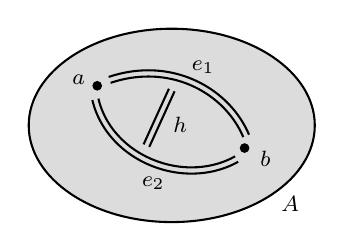
\begin{tikzpicture}[x=0.75pt,y=0.75pt,yscale=-1,xscale=1,roundnode/.style={circle, fill=black, inner sep=0pt, minimum size=3.5pt}]
    %uncomment if require: \path (0,300); %set diagram left start at 0, and has height of 300

    %Shape: Ellipse [id:dp3643970014729053] 
    \draw  [fill={rgb, 255:red, 220; green, 220; blue, 220 }  ,fill opacity=1 ] (4,52.08) .. controls (4,26.36) and (34.86,5.5) .. (72.92,5.5) .. controls (110.98,5.5) and (141.83,26.36) .. (141.83,52.08) .. controls (141.83,77.81) and (110.98,98.67) .. (72.92,98.67) .. controls (34.86,98.67) and (4,77.81) .. (4,52.08) -- cycle ;
    %Curve Lines [id:da06896022650610556] 
    \draw    (42.51,28.73) .. controls (49.06,26.53) and (55.48,25.53) .. (61.61,25.53) .. controls (81.63,25.53) and (98.59,36.2) .. (107.29,50.91) .. controls (108.37,52.74) and (109.33,54.63) .. (110.14,56.57)(43.46,31.57) .. controls (49.69,29.48) and (55.78,28.53) .. (61.61,28.53) .. controls (80.48,28.53) and (96.5,38.56) .. (104.71,52.44) .. controls (105.72,54.15) and (106.61,55.92) .. (107.38,57.73) ;
    %Curve Lines [id:da08140854638152761] 
    \draw    (37.58,39.19) .. controls (41.3,54.8) and (53.94,65.9) .. (68.57,70.27) .. controls (72.96,71.58) and (77.53,72.28) .. (82.1,72.31) .. controls (82.22,72.31) and (82.34,72.31) .. (82.46,72.31) .. controls (89.71,72.31) and (96.96,70.63) .. (103.45,66.99)(34.66,39.89) .. controls (38.64,56.55) and (52.07,68.48) .. (67.72,73.14) .. controls (72.37,74.53) and (77.23,75.28) .. (82.08,75.31) .. controls (82.2,75.31) and (82.33,75.31) .. (82.46,75.31) .. controls (90.22,75.31) and (97.97,73.5) .. (104.92,69.61) ;
    %Straight Lines [id:da7856762818241472] 
    \draw    (74.28,35.66) -- (62.08,62.46)(71.55,34.42) -- (59.35,61.22) ;

    \node[roundnode] (B0) at (37,33) {};
    \node (C0) at (28,30) {\footnotesize{$a$}};
    \node[roundnode] (B1) at (108,63) {};
    \node (C1) at (118,68) {\footnotesize{$b$}};
    \node (C2) at (88,24) {\footnotesize{$e_1$}};
    \node (C3) at (64,80) {\footnotesize{$e_2$}};
    \node (C4) at (77,52) {\footnotesize{$h$}};
    \node (C5) at (130,90) {\footnotesize{$A$}};
    \end{tikzpicture}
  \end{minipage}
  \begin{minipage}{0.4\textwidth}
  \[
    \begin{array}{l}
      A : \varType_i \\
      a : A \\
      b : A \\
      e_1 : \Indeq{A}{a}{b} \\
      e_2 : \Indeq{A}{a}{b} \\
      h : \Indeq{(\Indeq{A}{a}{b})}{e_1}{e_2}
    \end{array}
  \]
  \end{minipage}
  \caption{Représentation graphique d'un type avec des habitants et des égalités}
\end{figure}

Somme toute, avec l'axiome d'univalence les types ne se comportent plus 
tellement comme des ensembles. 
% 
Voevodsky a remarqué qu'ils ressemblent bien plus à des 
\emph{\( \infty \)-groupoïdes faibles}, un gadget catégorique qui joue un rôle 
important dans la théorie de l'homotopie, la branche des mathématiques qui 
étudie les espaces et leurs déformations. 
% 
C'est le point de départ de la \emph{théorie des types homotopique} (HoTT), une 
analogie profonde entre la théorie de l'homotopie et la théorie des types 
intensionnelle avec l'axiome d'univalence~\cite{hottbook}.

Lorsque nous faisons de la théorie des types homoptopique, nous considérons les 
types comme des espaces. Les habitants d'un type jouent le rôle de points, 
les égalités entre deux termes correspondent aux chemins entre les points, les 
égalités entre deux égalités sont des déformations continues entre les chemins 
correspondants, et ainsi de suite. 
% 
Logiquement, les fonctions entre deux types sont continues (car elles
préservent les égalités), et les isomorphismes correspondent aux équivalences 
d'homotopie. 

La théorie des types par homotopie étend également la notion de type inductif 
aux \emph{types inductifs supérieurs} (abrégés en HITs pour \emph{higher inductive types}), 
qui comportent des constructeurs de chemins/égalités en plus des constructeurs d'éléments. 
% 
Les HIT fournissent des outils pour construire des espaces basiques comme le cercle, 
la sphère et le tore, mais également de quoi former des types quotients.
% 
\sideremark{La définition du type \textsf{circle} peut être surprenante au premier 
  abord, car elle ne ressemble absolument pas à l'espace attendu
  \( \{ (x, y) \in \mathbb{R}^2\ |\ x^2 + y^2 = 1 \} \).
  En effet les types en HoTT ne correspondent pas à des espaces \emph{topologiques}, mais 
  plutôt à une notion synthétique d'espaces construits à partir de points, de lignes, de
  faces de dimensions supérieures, \etc
  Ainsi le type \textsf{circle} est librement engendré par un point et 
  un chemin qui relie ce point avec lui-même.}
\[
\begin{array}{l}
\mathsf{Inductive}\enskip\mathsf{circle} : \varType_0\enskip := \\
\sep \quad \mathsf{base} \enskip : \enskip \mathsf{circle}\\
\sep \quad \mathsf{loop} \enskip : \enskip \Indeq{\mathsf{circle}}{\mathsf{base}}{\mathsf{base}} \\
\end{array}
\]
\[
\begin{array}{l}
\mathsf{Inductive}\enskip\mathsf{quotient}\ (A : \varType_i)\ (R : A \to A \to \varType_i) : \varType_i\enskip := \\
\sep \quad \mathsf{emb} \enskip : \enskip A \to \mathsf{quotient}\ A\ R \\
\sep \quad \mathsf{quo} \enskip : \enskip \Depfun[a\ b]{A}{R\ a\ b \to \Indeq{...}{\mathsf{emb}\ a}{\mathsf{emb}\ b}} \\
\end{array}
\]

En utilisant des types inductifs supérieurs et l'axiome d'univalence, il devient
possible de prouver un nombre surprenant de résultats classiques de la théorie 
de l'homotopie, reformulés pour parler de types et d'égalité : 
% 
dans sa thèse, Brunerie a réussi à montrer que le quatrième groupe d'homotopie 
de la sphère tridimensionnelle a deux éléments~\sidecite{Brunerie16}. 
% 
Depuis lors, la communauté HoTT a développé des bibliothèques de 
mathématiques univalentes conséquentes, à l'aide des assistants de preuve
\Coq~\sidecite{Bauer:2017:HLF:3018610.3018615} et \Agda~\sidecite{agda-unimath}.

Toutefois, la théorie des types homotopique n'est pas une théorie qui 
\emph{calcule}. L'axiome d'univalence est un axiome (comme le nom l'indique!), 
ce qui signifie que l'éliminateur \( \mathsf{J} \) se contente de produire un 
terme bloqué lorsqu'il est appliqué à une égalité obtenue à partir d'un 
isomorphisme. 
% 
Les types inductifs supérieurs ne sont pas compatibles avec le calcul non plus, 
car leurs principes d'élimination sont postulés comme des axiomes. 
% 
Cette situation est d'autant plus décevante que les fonctionnalités introduites 
par HoTT semblent respecter les principes des mathématiques constructives.

\paragraph*{La Théorie des Types Cubique}
% 
Suite aux travaux de Voevodsky, la communauté des théoriciens des types
s'est penchée sur la question du comportement calculatoire de l'égalité 
univalente.

En 2014, Bezem Coquand et Huber ont construit le premier modèle de l'axiome d'univalence 
dans une théorie des ensembles constructive~\sidecite{BezemCoquandHuber14}.
% 
Leur modèle interprète les types comme des \emph{ensembles cubiques fibrants}, un 
objet combinatoire utilisé pour modéliser les \( \infty \)-groupoïdes faibles qui se prête 
bien à une présentation constructive. 
% 
Bien que le modèle de Bezem \etal ne comporte rien qui puisse ressembler à une 
règle de calcul, les ensembles cubiques se sont avérés être une manière fructueuse
de réaliser le potentiel constructif de l'univalence.

Ce programme s'est concrétisé un an plus tard avec l'introduction de la 
\emph{théorie des types cubiques}, une théorie des types intensionnelle enrichie 
avec les idées apportées par les ensembles cubiques fibrants~\sidecite{cubicaltt}.
% 
Ce nouveau système incorpore des primitives homotopiques directement dans les 
jugements de typage, et les équipe avec des règles de calcul adéquates. 
% 
Grâce à cette structure supplémentaire, il devient possible de prouver 
l'univalence comme un théorème, ce qui fait de la théorie des types cubiques une théorie 
univalente sans axiome.
% 
Étant donné qu'elle satisfait une propriété de canonicité~\sidecite{Huber16} et admet 
une fonction de normalisation pour les termes ouverts~\sidecite{sterling_normalization_cubical}, 
la théorie des types cubique fournit une réponse solide à la question du comportement 
calculatoire de l'univalence.
% 
En plus de cela, elle peut être étendue par des types inductifs supérieurs avec des 
principes d'élimination et des règles de calcul naturels~\sidecite{CavalloHarper19}.

Dans les années qui ont suivi son introduction, la théorie des types cubiques a 
évolué en un domaine de recherche dynamique. 
% 
De nombreuses variante du système original ont été étudiées sous un angle 
théorique~\cite{AngiuliHouHarper18,ABCFHL} et implémentées dans des assistants de 
preuve~\cite{Cubicaltt, redtt}. 
% 
Parmi celles-ci, le mode \texttt{cubical} d'\Agda est sans aucun doute l'implémentation 
qui a rencontré le plus franc succès, avec plusieurs projets de formalisation de 
grande envergure.

\section{Contributions}

\paragraph{Le Calcul des Constructions Observationnel}
% 
Dans la première partie de cette thèse, nous étudions les propriétés méta-théoriques 
de l'égalité observationnelle. 
% 
Pour ce faire, nous introduisons un calcul formel basé sur la théorie des types 
observationnelle d'Altenkirch \textit{et al}, que nous appelons le calcul 
des constructions observationnel (abrégé en \SetoidCC). 
% 
\SetoidCC possède des types dépendants avec des types inductifs et un univers 
imprédicatif de propositions strictes. 
% 
En plus de cela, on ajoute une implémentation de l'égalité observationnelle 
et un opérateur primitif de \emph{type-castring} à partir desquels nous pouvons 
dériver les principes d'unicité des preuves d'identité, d'extensionnalité des 
fonctions et d'extensionnalité des propositions.
% 
\SetoidCC permet également la formation de quotients d'un type par une relation 
d'équivalence stricte.

Nous équipons notre système formel d'une stratégie de réduction que nous utilisons 
pour prouver un théorème de normalisation, la canonicité des types de données de 
base et la décidabilité de la relation de typage. 
% 
Ces résultats sont obtenus grâce à un modèle de normalisation, que nous construisons 
dans \Agda en utilisant le cadre des relations logiques développé par Abel 
\etal~\sidecite{Abel:POPL2018}. 
% 
La preuve de normalisation peut être consultée en ligne \refAgdaRoot{Everything}, 
et des liens vers le code seront fournis à intervalles réguliers dans les chapitres 
correspondants.

À notre connaissance, notre modèle introduit plusieurs innovations par rapport 
à la littérature existante sur les preuves de normalisation. 
% 
La plus basique, mais aussi la plus importante, est que nous ne normalisons pas 
les preuves de propositions strictes, contrairement à l'approche défendue par 
Gilbert et al \etal~\sidecite{gilbert:hal-01859964}. 
% 
Cela nous permet non seulement de supporter les axiomes \emph{proof-irrelevant}, 
mais aussi de gérer l'imprédicativité sans avoir recours aux candidats de 
réductibilité usuels. 
% 
Comme nous n'avons pas besoin des candidats de réductibilité, nous pouvons 
utiliser une relation logique \emph{proof-irrelevant} pour notre preuve, ce 
qui nous permet d'ajouter des opérateurs non paramétriques tels que l'égalité 
observationnelle et le \emph{type-casting}. 
% 
En échange de cette flexibilité, notre refus de normaliser les preuves de
proposition a pour conséquence que la normalisation n'implique pas directement 
la canonicité, et qu'une preuve de cohérence séparée est nécessaire pour 
obtenir la canonicité---comme suggéré par McBride \etal dans leur article sur 
la théorie des types observationnelle~\sidecite{AltenkirchMcBrideSwiestra07}. 
% 
Nous réparons cette lacune en construisant un modèle de \SetoidCC en théorie 
des ensembles. 

Ce travail résout plusieurs problèmes qui étaient encore ouverts à notre 
connaissance : tout d'abord, nous obtenons une preuve complète de la 
normalisation et de la décidabilité pour la théorie des types observationnelle, 
déjà conjecturée par Altenkirch \etal. 
% 
De plus, l'égalité de \SetoidCC vit dans une sorte imprédicative de propositions 
strictes, tout comme l'égalité de \Lean. 
% 
Nous montrons que nous pouvons interpréter l'éliminateur J de \Lean dans une 
extension de \SetoidCC, tout en préservant la normalisation et la décidabilité 
du typage. 
% 
Ceci répond à la question d'Abel et Coquand sur la compatibilité de 
l'imprédicativité et de l'étalité en tant que proposition stricte~\sidecite{lmcs:6606}.

\paragraph{Vers une Traduction Cubique}
% 
Dans la deuxième partie, nous étudions la possibilité d'une traduction de 
\HoTT dans notre calcul des constructions observationnel. 
% 
Puisque \SetoidCC est un système calculatoire, une telle traduction fournirait 
une nouvelle façon de calculer avec l'axiome d'univalence. 

Le point de départ de cette partie est la traduction dite ``préfasciste'' 
de Pédrot qui interprète les types de la théorie de Martin-Löf comme des
préfaisceaux dans une théorie des types intensionnelle avec des propositions 
strictes~\sidecite{pedrot:prefascist}. 
% 
Les préfaisceaux sont une construction catégorique qui généralise de nombreux 
objets algébriques, y compris les ensembles cubiques que Coquand \etal ont 
utilisé pour modéliser l'univalence. 
% 
Cependant il manque un ingrédient important à la traduction préfasciste
comparé au modèle de Coquand \etal : les \emph{structures de fibration}.

Nous ajoutons deux nouvelles pierres à cet édifice : dans un premier temps, 
nous présentons une dissection de la construction préfasciste de Pédrot, 
en expliquant comment elle contourne les difficultés bien connues des 
préfaisceaux en théorie des types intensionnelle.
% 
Dans un second temps, nous expliquons comment étendre la traduction préfasciste 
avec une notion de structure de fibration qui devrait permettre une interprétation 
de l'axiome d'univalence.

\paragraph{Homotopie Synthétique en Théorie des Types Cubique}
% 
Enfin, dans la troisième partie de cette thèse, nous cherchons à montrer les 
avantages pratiques du calcul dans l'utilisation d'un système univalent.
% 
Pour ce faire, nous formalisons plusieurs résultats classiques de la théorie 
de l'homotopie en théorie des types cubiques, et nous comparons les preuves 
obtenues avec des formalisations analogues qui postulent l'univalence et les
HITs en tant qu'axiomes. 
% 
Notre panel de résultats inclut :
%
\begin{itemize}
\item L'équivalence entre le tore et le produit cartésien de deux cercles,
  avec un calcul de leurs groupes fondamentaux respectifs.
\item L'équivalence entre une définition directe des sphères de basses 
  dimensions et une définition alternative à base de suspensions itérées.
\item La définition du pushout homotopique avec une preuve directe du lemme
  ``\( 3 \times 3 \)''
\item La définition du joint de deux type et une preuve d'associativité. 
  Avec ces éléments, nous obtenons deux preuves différentes que la sphère $\Sp^3$
  est équivalente au joint de deux cercles.
\item Une définition de la fibration de Hopf et une preuve que son espace total
  est équivalent à la sphère $\Sp^3$.
\end{itemize}

Ce travail a été formalisé dans l'assistant de preuves \Agda, et a été incorporé dans
la bibliothèque standard de cubical Agda~\sidecite{agda-cubical-library}.

\subsection{Publications}

Cette thèse s'appuie sur trois articles revus et publiés dans des conférences internationales:
\begin{itemize}
\item Le travail sur le développement de l'homotopie synthétique en théorie
  cubique des types a été présenté dans un article co-écrit avec Anders 
  Mörtberg et publié à CPP'20~\sidecite{cubical-homotopy}.
\item La construction d'une relation logique pour une version prédicative
  de la théorie des types observationnelle a été réalisée en collaboration
  avec Nicolas Tabareau, et a fait l'objet d'une publication à POPL'22~\sidecite{pujet:hal-03367052}.
  Cet article a été nommé ``distinguished paper''.
\item Le travail sur l'imprédicativité et son interaction avec l'égalité 
  observationnelle a égélement été réalisé en collaboration avec Nicolas
  Tabareau, et a été conditionnellement accepté à POPL'23. 
\end{itemize}
En plus de cela, la traduction cubique étudiée en partie 2 a été l'objet d'un
\emph{extended abstract} presenté à ICMS'20.

\section{Théories et Méta-Théories}

Dans les chapitres suivants, nous manipulerons un certain nombre de systèmes formels---principalement 
des théories de types dépendantes, mais également quelques théories 
du premier ordre. 
% 
Comme la correspondance entre les théories des types et les noms semble varier
significativement d'un auteur à l'autre, nous fixons notre propre convention :

\begin{tabular}{p{3em} p{0.82\textwidth} }
\MLTT & 
  La Théorie des Types Intensionnelle de Martin-Löf désigne un système avec des 
  produits dépendents, une hiérarchie prédicative d'univers et une \emph{certaine quantité} de 
  types inductifs~\cite{MartinLoef75}.
  % 
  Nous demeurons intentionnellement vagues au sujet des types inductifs.
  Lorsque les inductifs jouent un rôle important, nous utiliserons des notations plus explicites
  que nous introduirons au besoin.
\end{tabular}

\begin{tabular}{p{3em} p{0.82\textwidth} }
\CIC & 
  Le Calcul prédicatif des Constructions Inductives étend \MLTT 
  avec une sorte imprédicative \( \varProp \), qui supporte l'élimination large 
  des types inductifs sous-singletons~\cite{Paulin15}.
\end{tabular}

\begin{tabular}{p{3em} p{0.82\textwidth} }
\SetoidCC / \SetoidCCplus & 
  Le Calcul des Constructions Observationnel désigne notre implémentation de 
  la théorie des types observationnelle de McBride \etal 
  Une présentation détaillée est donnée dans le chapitre \ref{ch:observational}.
  % 
  Le système étendu \SetoidCCplus ajoute une règle supplémentaire pour le calcul
  du \emph{type-casting} sur les preuves d'égalité réflexives, comme décrit dans le 
  chapitre \ref{ch:extensions}. 
\end{tabular}

Comme la majeure partie de cette thèse traite des propriétés méta-théoriques 
des théories des types, nous les traiterons généralement comme des objets 
mathématiques, c'est-à-dire comme une collection de lexèmes
et de règles de typage. 
% 
Mais les théories des types sont également des théories mathématiques à part 
entière, que nous pouvons utiliser pour prouver des théorèmes.

Et en effet, nous développerons beaucoup de mathématiques à l'intérieur de 
théories des types, en adoptant généralement un style informel pour éviter 
de submerger le lecteur avec des termes de preuve peu lisibles. 
% 
Lorsque nous utilisons la théorie des types comme méta-théorie, nous utilisons 
la syntaxe et le schéma de couleurs de l'assistant de preuve \Agda, pour la 
simple raison que toutes nos formalisations sont effectuées en \Agda. 
% 
Si aucun code en \Agda n'apparaît, il est raisonnable de supposer que nous travaillons 
sans présupposer une méta-théorie précise, comme c'est le cas dans la majorité
de la littérature mathématique.
